\section{Antecedentes y marco teórico}
\label{sec:antecedentes_marco_teorico}
\subsection{Tomografía óptica de coherencia}

En lo últimos años han aparecido nuevas técnicas para la toma de imágenes en múltiples disciplinas científicas, entre ellas destacan por su alta actividad de investigación, la formación de imágenes biomédicas, impulsado principalmente por el constante desarrollo de dispositivos para telecomunicaciones que han permitido la producción de instrumentos electromagnéticos de alto desempeño a costos relativamente bajos. Como consecuencia de esto, múltiples técnicas para el escaneo materiales altamente dispersivos, como los tejidos biológicos han sido creadas. De estas técnicas surge la tomografía, que es particularmente interesantes por su potencial para realizar imágenes que ayudan al diagnóstico médico a través de exámenes \emph{no invasivos}. La tomografía en general se basa en la creación de ``cortes''  de objetos tridimensionales, que en conjunto generan una imagen en dos o tres dimensiones de la muestra en cuestión. \emph{La OCT es una técnica no invasiva de imagen tridimensional capaz de producir imágenes con alta resolución lateral y axial a través de muestras dispersivas e inhomogéneas, tales como los tejidos biológicos} \cite{Tomlins}. En sus inicios, las técnicas de OCT se basaron en medidas de profundidad de baja coherencia en el dominio temporal con un interferómetro de luz blanca. La posibilidad de emplear interferómetros de luz blanca para la formación de imágenes tridimensionales en tejidos biológicos fue liderada por Huang \etal en 1991 \cite{Huang1991}, quienes propusieron emplear reflectometría de baja coherencia en sistemas biológicos. Su sistema de OCT se basa en múltiples escaneos de una serie de ubicaciones laterales y axiales para proveer un mapa de sitios o lugares en donde la muestra refleja luz. Una de las características más importantes de esta nueva técnica, es que a diferencia de la microscopía confocal, en donde la resolución longitudinal depende de la apertura numérica, en OCT la resolución solo está limitada por la longitud de coherencia de la fuente de luz, por consiguiente, OCT puede tener alta resolución en profundidad aun si la apertura del sistema es pequeña.

\subsection{El papel de la OCT en imagen médica}

La OCT tiene diversos aspectos que son comunes al ultrasonido y a la microscopía. Por un lado, la resolución en imágenes de ultrasonido de alta resolución, se encuentra en el rango típico de $0.1$ hasta $1mm$ y dependerá de la frecuencia de la onda de sonido que se emplee, los valores típicos para la frecuencia varían entre los $3$ y $40MHz$ \cite{Szabo}. Sin embargo, en este rango de frecuencias es difícil emplear las ondas de sonido en tejidos, ya que éstos además de ser altamente dispersivos, atenúan fuertemente las ondas en unos pocos milímetros. Por otro lado, algunas ramas de la microscopía poseen una alta resolución en imagen de tejidos, por ejemplo, la microscopía confocal, cuya resolución es de alrededor de $1\mu m$ o inclusive menor. En la microscopía confocal, la resolución está limitada por la difracción, relacionada a su vez con la apertura numérica del sistema; y su capacidad de producir imagen se encuentra influenciada principalmente por la degradación de la luz en dispersiones no deseadas, lo que produce un bajo contraste en la señal a medir \cite{Pawley}. 

La OCT por su lado, llena un vacío de resolución entre el ultrasonido y la microscopía, ya que el rango en el cual se mueve la OCT varía entre $1$ y $15 \mu m$, aproximadamente $100$ veces más fino que el ultrasonido, como se presenta en la Fig.~\ref{fig:OCT_Ultrasound_microscopy}. La principal limitación en OCT se encuentra en que la luz es altamente dispersada por muchos tejidos, lo que limita la profundidad de penetración a $\sim 2mm$ en muchos casos.
%Mientras que una de sus principales ventajas está en su fácil integración en instrumentos médicos, tales como catéteres, endoscopios, laparoscopios o incluso, agujas quirúrgicas que permite hacer imagen de órganos, o incluso, tejidos sólidos en el cuerpo.

\begin{figure}[ht!]
	\centering
	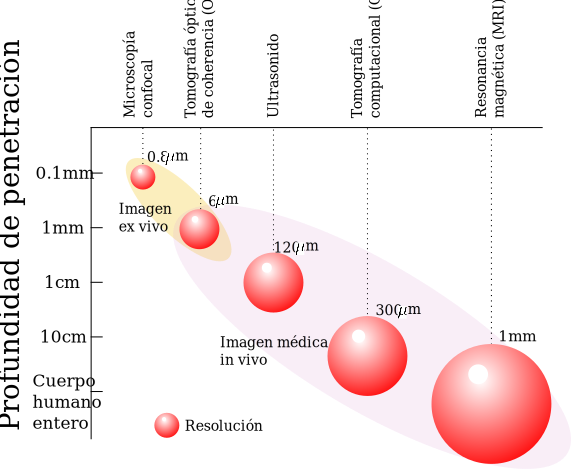
\includegraphics[width = 0.7\textwidth, keepaspectratio]{img/Carlos_oct_resolucion}
	\caption{Comparación de la resolución contra la profundidad de penetración de diferentes modalidades de imagen médica.}
	\label{fig:OCT_Ultrasound_microscopy}
\end{figure}


La OCT es análoga al ultrasonido con la diferencia de emplear luz en lugar de sonido, su principio básico se centra en medir la magnitud y el tiempo de retraso (``eco'') que producen las ondas al llegar a la muestra, de forma que las retrodipersiones o retroreflecciones en diferentes distancias permite determinar el tamaño y reconstruir microestructuras \cite{Szabo}. Como la velocidad del sonido es de alrededor de $1300m/s$, el ultrasonido ha impulsado la creación de sensores y métodos de sensado que permitan una alta tasa de recepción de información, lo que a su vez ha incentivado el desarrollo de equipos para OCT, en especial si se considera que la luz viaja a $3\times 10^8 m/s$ y que las tasas de recepción de datos deben de ser mayores. Una de las principales ventajas de la analogía OCT/ultrasonido se encuentra en su fácil integración en instrumentos médicos, tales como catéteres, endoscopios, laparoscopios o incluso, agujas quirúrgicas que permite hacer imagen de órganos o tejidos sólidos \invivo en el cuerpo humano~\cite{Tearney1996, Tearney1997_2}.

%La OCT es análoga al ultrasonido, con la diferencia de emplear luz en lugar de sonido. El principio básico de la OCT, es medir la magnitud y el retraso de las retrodipersiones o retroreflecciones de la luz en microestructuras en tejidos, de forma que el tamaño de las microsestructuras puede determinarse a través de la medida del tiempo que tarda el ``eco'' del sonido o la luz en viajar diferentes distancias. El desarrollo de equipos para tratamientos con ultrasonido a su vez ha posibilitado la creación de equipos de bajo costo para OCT, en especial si se considera que la velocidad del sonido es de alrededor de $1300m/s$, mientras que la luz viaja a $3\times 10^8 m/s$. Una de las principales ventajas de la analogía OCT/ultrasonido se encuentra en su fácil integración en instrumentos médicos, tales como catéteres, endoscopios, laparoscopios o incluso, agujas quirúrgicas que permite hacer imagen de órganos o tejidos sólidos \invivo en el cuerpo.

\subsection{Los inicios de la OCT}

%La propuesta de la técnica de OCT surgió hacia el año 1991 por Huang \etal \cite{Huang1991}, sus primeras pruebas fueron realizadas \emph{ex vivo} en la retina y la arteria coronaria. Huang \etal proponen una técnica análoga al ultrasonido, pero que en lugar de emplear ondas de sonido, emplea luz para realizar reconstrucciones tridimensionales a partir de escaneos bidimensionales, a esta técnica la denominarían tomografía óptica de coherencia, y se basa esencialmente en el empleo de un interferómetro de luz blanca. Con los resultados obtenidos por Huang \etal la OCT se ha posicionado como una de las más grandes aplicaciones emergentes para el diagnóstico oftalmológico e intravascular.

La propuesta de OCT surgió hacia el año 1991 por Huang \etal \cite{Huang1991}, sus primeras pruebas fueron realizadas \exvivo en la retina y la arteria coronaria, y desde estos resultados pudo verse la utilidad de OCT para el diagnóstico oftalmológico e intravascular, áreas en las que ha tenido grandes avances. El ojo humano puede ser analizado ópticamente, es decir, es posible implementar técnicas para observar de manera directa la zona interior del ojo, lo que ha impulsado el uso de métodos de imagen en oftalmología; muchos de los primeros estudios realizados con OCT fueron basados en el ojo humano. Las primeras imágenes \invivo de la retina fueron obtenidas de manera independiente por Fercher \etal \cite{Fercher1993} y Swanson \etal \cite{Swanson1993} en 1993. Estos resultados conllevaron a que en la década de los 90 se diera un alto uso de OCT para el monitoreo, seguimiento, detección y diagnosis de diferentes enfermedades, entre las cuales destaca: enfermedades maculares \cite{Puliafito1995}, incluyendo agujeros maculares \cite{Hee1995_2} y edemas maculares \cite{Hee1995},  coriorretinopatía serosa central \cite{Hee1995_3}, y degeneraciones maculares asociadas a la edad y a la neovascularización coroidal \cite{Hee1995_4}. Un ejemplo de monitoreo con OCT, está en el espesor de las capas de fibra del nervio retinal, el cual es un indicador de glaucoma, y que puede cuantificarse en ojos normales y con glaucoma. Mediante una correlación con medidas convencionales de la estructura y función del nervio óptico, es posible encontrar focos de glaucoma, trabajo realizado también a partir de la OCT en 1995 por Schuman \etal \cite{Schuman1995}.

La alta sensibilidad de la OCT permite producir imagen de estructuras tales como la retina, que poseen un bajo índice de dispersión de la luz, sin embargo, la mayor parte de las aplicaciones que emplean OCT requieren la captura de imágenes en tejidos que no son transparentes y además, son altamente dispersivos. En estos casos, es cuando la sensibilidad del método se vuelve relevante, ya que como la señal es fuertemente atenuada por la dispersión, la sensibilidad es quien determina la profundidad hasta la cual se puede conseguir imágenes \cite{Drexler2015}. Las primeras imágenes de tejidos diferentes al ojo, fueron posibles mediante el estudio de la influencia de la longitud de onda en la dispersión de la luz, en done se obtuvo que longitudes de onda más largas que el visible, reducen la dispersión producida por las muestras biológicas e incrementa la profundidad de penetración de la imagen \cite{Brezinski1996, Schuman1995}. Uno de los primeros estudios del efecto de la longitud de onda sobre las reconstrucciones con OCT fue realizado por Brezinski \etal \cite{Brezinski1996}, quienes realizaron una comparación de imágenes capturadas a $850$ y $1300nm$ \exvivo en una epiglotis humana. La imagen tomada a $1300nm$ mostró una mayor penetración puesto que los principales absorbentes en la mayor parte de los tejidos son la melanina y la hemoglobina, los cuales poseen una alta absorción en el visible y el infrarojo cercano \cite{Parsa1989}, mientras que la absorción del agua se convierte en dominante para mayores longitudes de onda, alrededor de los $1800-2000nm$. Por otro lado, en la mayoría de los tejidos, la dispersión en las longitudes de onda del infrarrojo cercano es uno o dos órdenes de magnitud mayores que la absorción, y la dispersión disminuye para longitudes de onda más grandes.

%\begin{figure}[ht!]
%\centering
%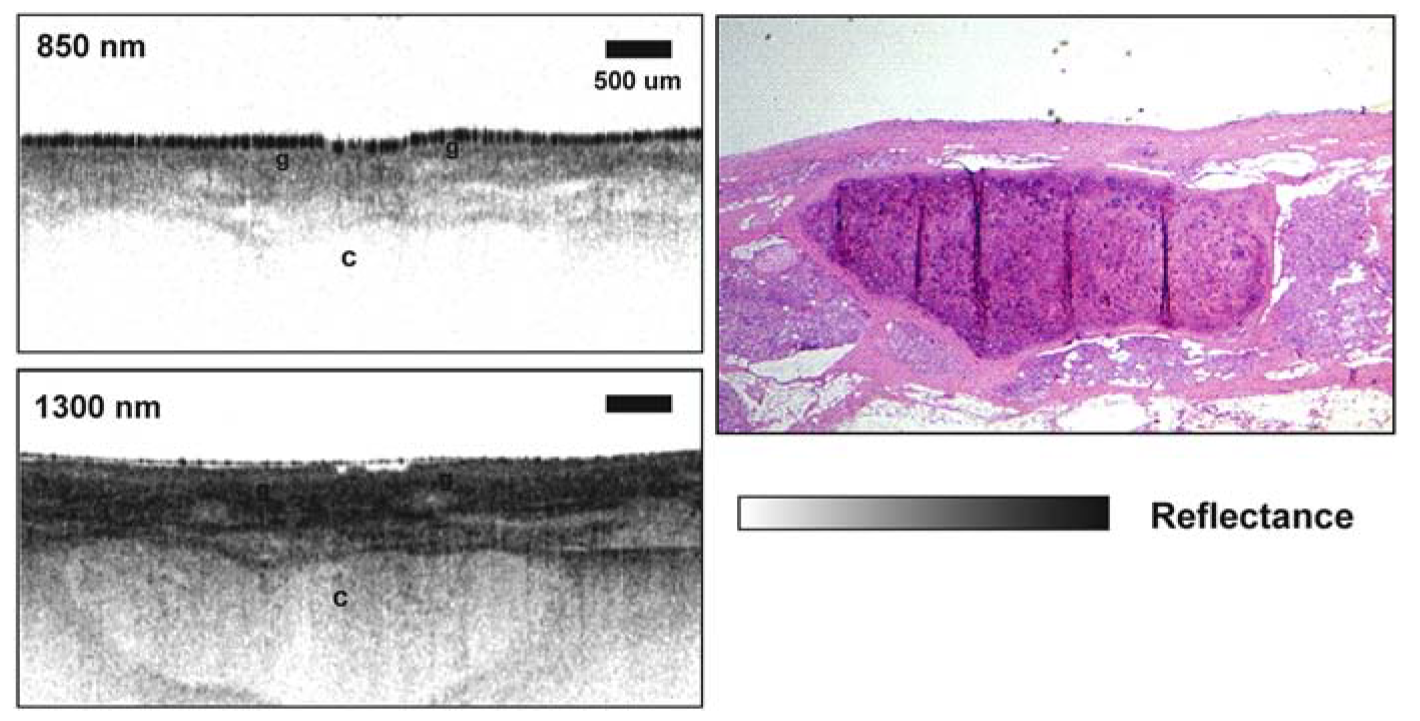
\includegraphics[width = \textwidth, keepaspectratio]{img/oct_longitudes_multiples.png}
%\caption[OCT empleando diferentes longitudes de onda.]{Profundidad de penetración de la OCT en diferentes longitudes de onda. Comparación de la atenuación producida por diferentes longitudes de onda en OCT, visualmente se aprecian más detalles cuando se emplea una longitud de onda de $1300nm$ que con $850nm$. Tomado de \cite{Brezinski1996}.}
%\label{fig:oct_longitudes_multiples}
%\end{figure}

Muchos estudios iniciales de la OCT se realizaron \exvivo en especímenes quirúrgicos, estos estudios fueron útiles para definir las estructuras que serían posibles de observar usando OCT \cite{Brezinski1996} y compararlo con la histología \footnote{estudio de la composición, estructura y características de los tejidos orgánicos de los seres vivos}. El estudio de la correlación entre las imágenes \exvivo de la  OCT y la histología se extendió a estudios hasta de enfermedades gastrointestinales \cite{Izatt1996, Tearney1997, Kobayashi1998, Pitris2000}, biliares \cite{Tearney1998}, en el aparato reproductor femenino \cite{Pitris1999}, pulmonares \cite{Pitris1998} y urinarias \cite{Tearney1997}.


\subsection{OCT: esquema}
\label{sec:OCT_Esquema}

\emph{La OCT es una técnica interferométrica que se basa en la interferencia de un campo óptico de banda ancha, es decir, que recoge múltiples longitudes de onda, el cual se divide y posteriormente se combina, produciendo interferencia únicamente en la región del espacio en el cual la diferencia de camino óptico se encuentra dentro de la longitud de coherencia} \cite{Fercher}. Un esquema típico de OCT se muestra en la Fig. \ref{fig:OCT_Scheme}. 

\begin{figure}[ht!]
	\centering
	\includegraphics[width = 0.5\textwidth, keepaspectratio]{img/Carlos_oct_Scheme}
	\caption{Esquema básico de la OCT, un interferómetro de Michelson se emplea para producir interferencia de baja coherencia entra el haz objeto y referencia.}
	\label{fig:OCT_Scheme}
\end{figure}

El esquema de la OCT se basa esencialmente en un interferómetro de Michelson que funciona de la siguiente forma: Primero un haz que proviene de una fuente viaja a través de un divisor de haz. Los haces divididos a su vez van por dos caminos diferentes, la porción del haz de referencia se refleja en un espejo, mientras que la otra porción del haz es enviada hacia la muestra, en donde se refleja desde diferentes profundidades al interior de la muestra. \emph{Como el haz posee una banda ancha, la interferencia entre el campo óptico de referencia y el que es reflejado por la muestra solo puede ser observado cuando ambos brazos tengan diferencias de camino óptico que se encuentren dentro de la longitud de coherencia del haz. Por consiguiente, la resolución axial de un sistema de OCT está determinado por la coherencia temporal de la fuente de luz}. En OCT, la longitud de coherencia $l_c$ se define como:

%Si la diferencia de camino óptico entre ambos brazos se encuentra dentro de la longitud de coherencia, se define el tamaño de ida y vuelta de longitud de coherencia $l_c$  como:

\begin{equation}
	\label{eq:l_c}
	l_c = \frac{2\ln 2}{\pi} \frac{\bar{\lambda}}{\Delta \lambda},
\end{equation}

\noindent donde $\bar{\lambda}$ es la longitud de onda central y $\Delta \lambda$ es el ancho del espectro (banda), $l_c$ indica la condición para la cual es posible obtener interferencia y por tanto la distancia axial mínima que puede medirse en OCT. \emph{Los objetos aparecen cuando se dan cambios precipitados en el índice de refracción entre profundidades o capas cercanas en la muestra, y se manifiestan como picos de intensidad en el patrón de interferencia}, nótese que la intensidad medida es aquella que proviene de la retrodispersión causada por la muestra. Debido a que el espectro es ancho, otra posibilidad de medir la información de profundidad en la muestra, es a través de las transformadas de Fourier, realizando mediciones sobre el dominio de las frecuencias y transformando el espectro de salida. En este caso, el haz de referencia permanece en una posición fija y las componentes frecuenciales de la OCT se detectan mediante un espectrómetro \cite{Drexler2015,Brezinski2005}.

En OCT pueden realizarse escaneos bidimensionales si no se modifica la diferencia de camino, o escaneos tridimensional a través de la medición de diversas profundidades en la muestra, que pueden ser realizadas mediante escaneos laterales del haz en una o dos direcciones ortogonales. Valores típicos de escaneos para profundidad pueden ir en $500$ profundidades distribuidas en una distancia de $3mm$ \cite{Tomlins}. Si el medio es turbio, las profundidades obtenidas en la literatura han sido entre $1$ y $3mm$, empleado longitudes de onda entre $800$ y $1300nm$ \cite{Drexler2015}.

Por último, algunas propiedades que cabe resaltar sobre OCT son las siguientes:
\begin{itemize}
	\item Alta resolución en imagen de profundidad.
	\item Resolución en profundidad, con distancias que van desde $1\mu m$ hasta $5mm$.
	\item Alta sensibilidad, permitiendo la captura de muestras poco dispersivas incluso en medios turbios.
	\item OCT no es una técnica invasiva, que posibilita su uso \invivo e \emph{in-situ}.
\end{itemize}

\subsection{Interferometría de baja coherencia}

Considere un intereferómetro de Michelson, como se muestra en la Fig.~\ref{fig:OCT_Scheme}, ese interferómetro es iluminado con una fuente de banda ancha, cuyo campo eléctrico $E_i$ puede expresarse en forma compleja como
\begin{equation}
	E_i(k,\omega) = s(k,\omega) e^{i(kz - \omega t)},
\end{equation}
donde $s(k,\omega)$ es la amplitud del campo eléctrico expresado como una función del número de onda $k = 2\pi /\lambda$ y de la frecuencia angular $\omega = 2\pi \nu$, que representan respectivamente la dependencia espacial y temporal de cada una de las componentes del espectro del campo con longitud de onda $\lambda$. La frecuencia y la longitud de onda se encuentran vinculadas por el índice de refracción del medio $n$ y la velocidad de luz en el vacío $c$, $\lambda \nu = c / n(\lambda)$, en medios dispersivos el índice de refracción depende de la longitud de onda. Se asume que el divisor de haz produce una división del campo incidente en dos componentes cada una con la mitad de la intensidad total, y adicionalmente es acromático. De los dos haces producidos por el divisor de haz, al que es reflejado cuando llega al divisor se le denota haz referencia, mientras que el que es refractado por el divisor haz objeto. El haz de referencia se propaga una distancia $z_R$ y nuevamente es reflejado por un espejo situado en $z = z_R$, el espejo de referencia tiene una reflectividad $r_R$ y la intensidad que refleja es $R_R = |r_R|^2$, finalmente, el haz reflejado regresar hasta el divisor de haz. 

El haz objeto por su parte, se propaga hasta llegar a la muestra. La muestra está caracterizada por tener una reflectividad de campo eléctrico dependiente de la profundidad $r_S(z_S)$, donde $z_S$ es la profundidad en la muestra medida desde el divisor de haz. En general, $r_S(z_S)$ es una función compleja que informa no solo la amplitud de la onda reflejada por la muestra, sino que además indica los cambios de fase que la onda puede experimentar. Adicionalmente, en el caso de especímenes biológicos, se trata de una función que refleja el cambio continuo del índice de refracción de los tejidos biológicos. Sin embargo, para entender el fenómeno de reflexión en la muestra, se asume que hay una serie de $N$ reflectores ubicados a lo largo de la muestra \footnote{Hay diferentes tratamientos que se basan en sistemas discretos y continuos, el último caso puede consultarse de manera detallada en \cite{Brezinski2005,Fercher}.}, de la siguiente forma, 

\begin{equation}
	r_S(z_S) = \sum_{n=1}^{N} r_{S_n} \delta[(z_S - z_{S_n})],
\end{equation}

\noindent donde $r_{S_1}, r_{S_2}, ..., r_{S_n}$ es el coeficiente de reflexión de campo eléctrico del $n$-simo reflector y $ z_{S_1}, z_{S_2}, ..., z_{S_n}$ es la distancia del $n$-simo reflector con respecto al divisor de haz. La intensidad reflejada por cada uno de los $n$ reflectores es $R_{S_n} = |r_{S_n}|^2$. \emph{El objetivo de OCT es poder identificar la función $\sqrt{R_{S}(z_S)}$ a través de medidas de interferométricas de baja coherencia}, lo que es la reflectividad de cada una de las profundidades en la muestra en estudio.



Luego de que el haz objeto y el haz referencia regresan al divisor de haz, el campo eléctrico reflejado corresponde a $E_R = \frac{E_i}{\sqrt{2}}r_Re^{i2kz_R}$ y $E_S = \frac{E_i}{\sqrt{2}} \sum_{n=1}^{N}r_{S_n} e^{i2kz_{S_n}}$ respectivamente. El factor exponencial surge por el cambio de fase que se produce durante la propagación, y la función $\delta$ del haz objeto ha sido incluida en el cambio de fase que se produce en la distancia $z_{S_n}$. Estos dos campo regresan hasta el divisor de haz y luego de atravesarlo tienen la mitad de su intensidad inicial, siguiendo su recorrido hasta llegar al detector, en donde se tiene la interferencia entre ellos $I(k,\omega)$, dada por

\begin{equation}
	I(k,\omega) = \frac{1}{2}|E_R+E_S|^2 = (E_R + E_S)(E_R + E_S)^{\ast},
\end{equation}

\noindent donde $^{\ast}$ representa la operación complejo conjugado. Si el patrón de interferencia $I(k,\omega)$ es registrado por un fotodetector, la fotocorriente que en este se produce es proporcional a la intensidad del patrón de interferencia multiplicado por un factor de respuesta propio del detector $I_D(k, \omega) = \rho \langle I(k, \omega) \rangle$, donde $\rho$ es el factor de respuesta del sensor y $\langle \cdot \rangle$ es la integración sobre el tiempo de respuesta. Reemplazando los valores anteriores, se puede expresar la corriente sensada por el detector como

\begin{equation}
\label{eq:Id}
	I_D(k, \omega) = \frac{\rho}{2} \bigg\langle \bigg| \frac{s(k, \omega)}{\sqrt{2}} r_R e^{i(2kz_R-\omega t)} + \frac{s(k, \omega)}{\sqrt{2}} \sum_{n=1}^{N} r_{S_n} e^{i(2kz_{S_n} - \omega t)} \bigg|^2 \bigg\rangle.
\end{equation}

Nótese que si se expande la Eq.~\ref{eq:Id}, los términos que son dependientes de $\omega$ se anulan y la expresión final es independiente del tiempo, esto tiene sentido si se considera que la frecuencia de la onda $\nu$ es mucho mayor que el tiempo de respuesta del detector. La Eq.~\ref{eq:Id} puede expresarse como

%La expresión simplificada de la Eq.~\ref{eq:Id} es
%
%\begin{align}
%\label{eq:ID_2}
%%	I_D(k) &= \frac{\rho}{4}\left[ S(k) (R_R + R_{S1} + R_{S2} + ...) \right] \notag \\
%	& + \frac{\rho}{4} \left[ S(k) \sum_{n=1}^{N} \sqrt{R_R R_{S_n}} \left( e^{i2k(z_R-z_{S_n})} + e^{-i2k(z_R-z_{S_n})} \right) \right] \\
%	& + \frac{\rho}{4} \left[ S(k) \sum_{m\neq n=1}^{N} \sqrt{R_{S_n}R_{S_n}} \left( e^{i2k(z_{S_n}-z_{S_m})} + e^{-i2k(z_{S_n}-z_{S_m})} \right) \right], \notag
%\end{align}
%
%\noindent donde $S(k) = \langle |s(k,\omega)|^2 \rangle$, que es la dependencia de $\lambda$ de la fuente. La Eq.~\ref{eq:ID_2} puede expresarse como

\begin{align}
\label{eq:ID_fin}
	I_D(k) &= \frac{\rho}{4}\left[ S(k) (R_R + R_{S1} + R_{S2} + ...+R_{Sn}) \right] \notag \\
	& + \frac{\rho}{2} \left[ S(k) \sum_{n=1}^{N} \sqrt{R_R R_{S_n}} \left( \cos[2k(z_R - z_{S_n})] \right) \right] \\
	& + \frac{\rho}{4} \left[ S(k) \sum_{m\neq n=1}^{N} \sqrt{R_{S_n}R_{S_m}} \left( \cos[2k(z_{S_n} - z_{S_m})] \right) \right], \notag
\end{align}

\noindent donde $S(k) = \langle |s(k,\omega)|^2 \rangle$ es la dependencia respecto a $\lambda$ de la fuente, es decir, su espectro. La Eq.~\ref{eq:ID_fin} posee tres miembros que corresponden a:

\begin{itemize}
	\item El primer término es independiente de la diferencia de camino óptico y actúa como un escalamiento de la señal en el detector. Es proporcional a la longitud de onda y a la reflectividad de la muestra y del espejo de referencia. Este término corresponde a la componente ``DC'' de la señal que se mide.
	\item El segundo término es la ``correlación cruzada'' de cada reflector en la muestra. Éste es dependiente tanto del número de onda y de la diferencia de camino entre el haz de referencia y el haz objeto. La señal que se desea medir con OCT proviene justamente de este término, aunque al ser proporcional a la raíz cuadrada de la reflectividad la magnitud de esta señal es bastante menor que la componente DC.
	\item El tercer término corresponde a la ``autocorrelación'' y representa la interferencia que ocurre entre los diferentes reflectores en la muestra y se conoce como ``artefactos'' en la señal.
\end{itemize}

%$$ \sqrt{R_R R_{S1}}  \sqrt{R_R R_{S3}} \sqrt{R_R R_{S4}} \lambda_0 /2 l_c$$

%Nótese que en la Eq.~\ref{eq:ID_fin} si solo se tuviera un reflector ($z_{S1}$), aparecería la señal DC, uno de los términos de interferencia y el espectro de la fuente $S(k)$ estaría solamente modulada por una función coseno, cuyo periodo es proporcional a la distancia entre la muestra y el espejo de referencia. Adicionalmente, la interferencia también es proporcional a la reflectividad del reflector $\sqrt{R_{S1}}$. En el caso en el cual hay múltiples reflectores, cada la interferencia se modula de acuerdo con la diferencia de camino entre los brazos, de forma que varias modulaciones aparecen sobre el espectro de la fuente.


En la Eq.~\ref{eq:ID_fin} si solo se tuviera un reflector ($z_{S1}$), la ecuación estaría regida por la componente DC de la señal y una modulación del espectro de la fuente $S(k)$ dependiente de una función coseno cuyo periodo es proporcional a la diferencia de camino óptico entre el haz objeto y referencia. Adicionalmente, la visibilidad del patrón de interferencia también es proporcional a la reflectividad $\sqrt{R_{S1}}$. Como lo muestra la Eq.~\ref{eq:ID_fin}, hay una relación directa entre la reflectividad de la muestra y el espectro de la fuente que se emplee. Para el caso de OCT, lo más común es emplear fuentes cuyo espectro posea una distribución gaussiana dadas las propiedades que esta posee, particularmente por el hecho de que la autocorrelación de una función gaussiana es otra función gaussiana. Si la fuente posee una distribución espacial $\gamma(z)$, tanto su transformada de Fourier (espectro $S(k)$) y su distribución espacial poseen la misma forma, con la diferencia de tener un ancho diferente, matemáticamente esto es
\begin{equation}
	\gamma (z) = e^{-z^2\Delta k^2} \leftrightarrow F\{\gamma (z)\} = S(k) = \frac{1}{\Delta k \sqrt{\pi}} e^{-\left[\frac{(k-k_0)}{\Delta k}\right]^2},
\end{equation}
\noindent donde $k_0$ es el número de onda central de la fuente $k_0 = 2\pi / \lambda_0$ y $\Delta k$ es el ancho de banda espectral.
%\begin{figure}[h!]
%	\centering
%	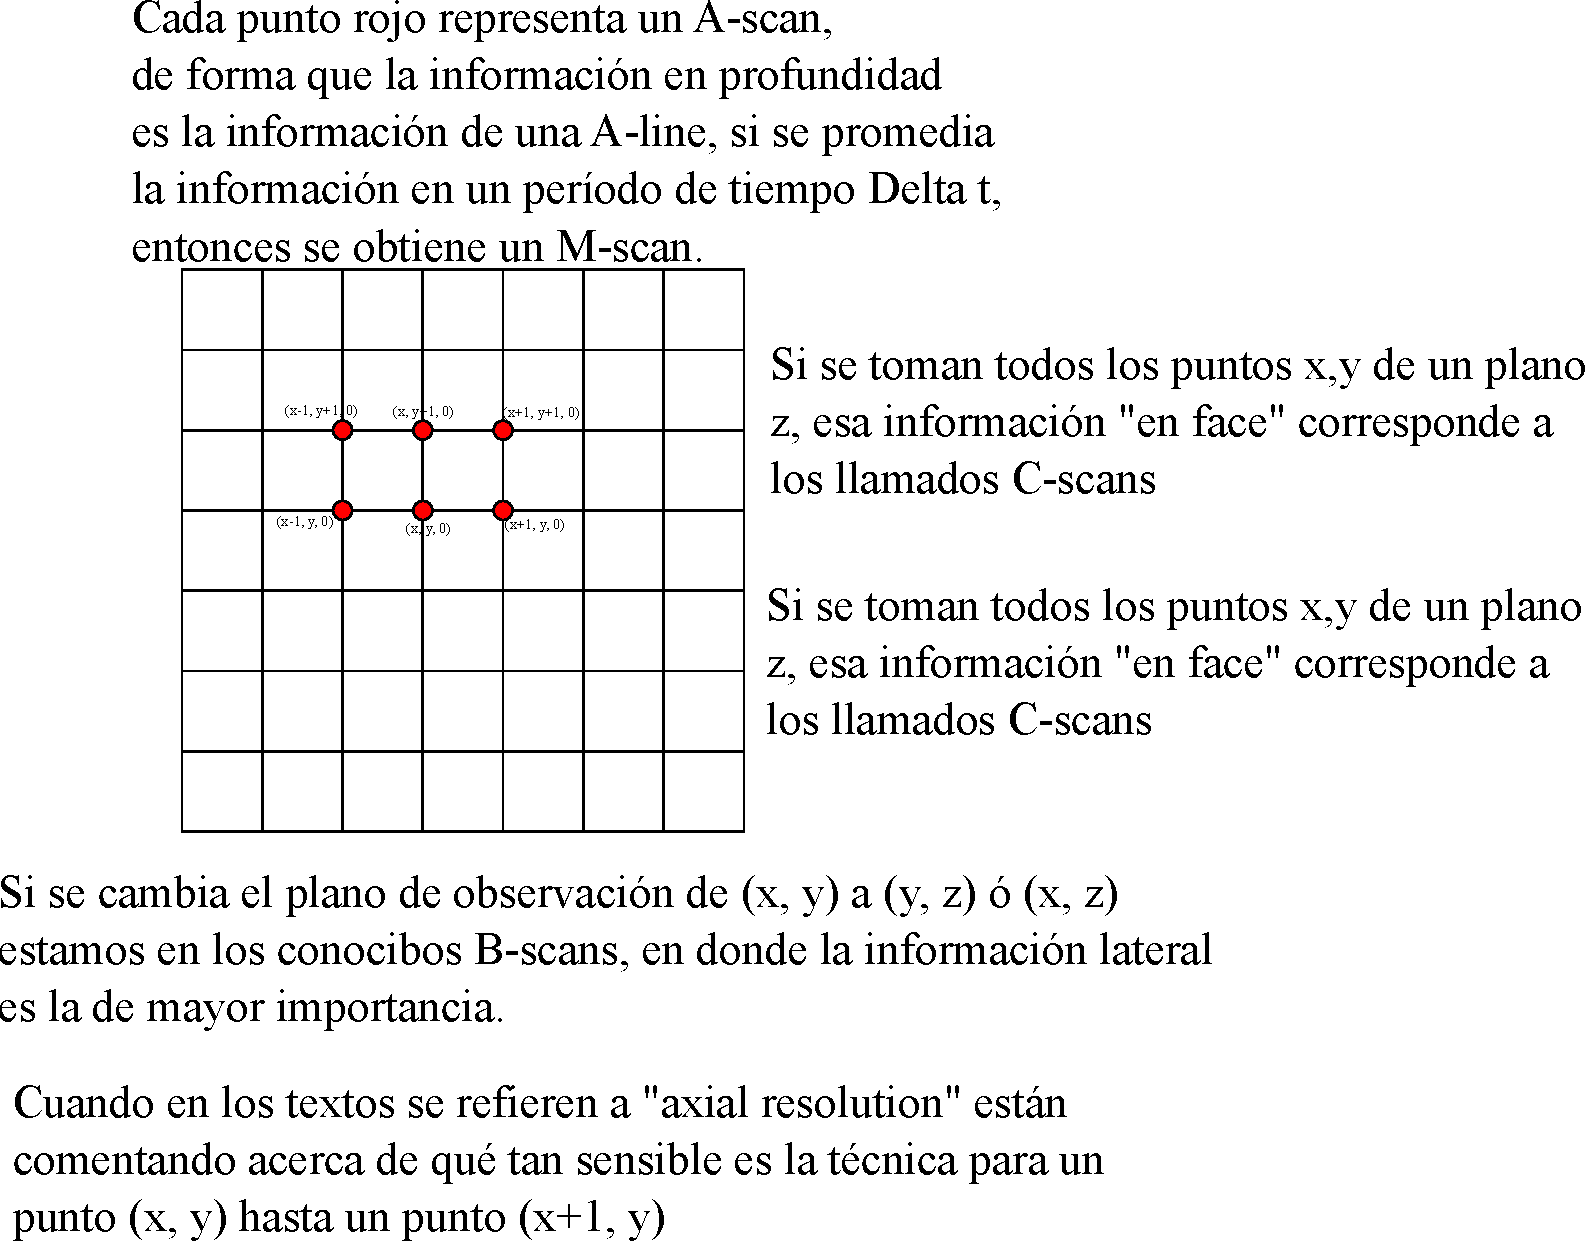
\includegraphics[width=0.7\linewidth]{img/a_scan.pdf}
%	\caption{Interpretación de la resolución axial, y los tipos de escaneos}
%	\label{fig:ascan}
%\end{figure}

%\begin{figure}
%\centering
%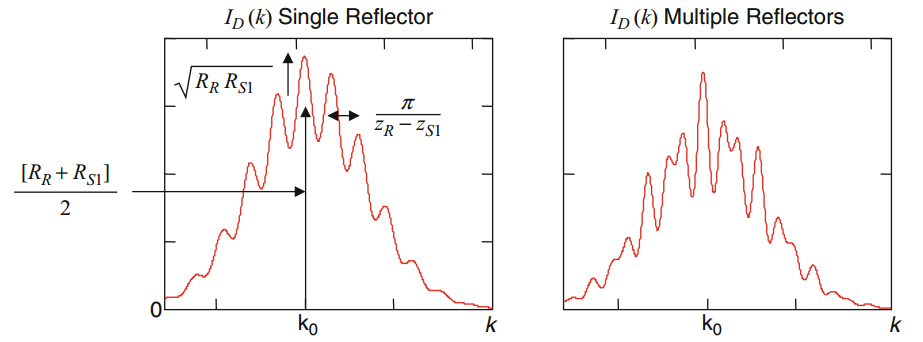
\includegraphics[scale=0.7]{img/gauss_reflect_oct.png}
%\caption{1}
%\label{fig:gaussreflectoct}
%\end{figure}

\subsection{Interferometría de baja coherencia en el dominio del tiempo}

%En la OCT en el dominio del tiempo TDOCT (\textit{time-domain optical coherence tomography}), el barrido no se realiza mediante el cambio del número de onda $k$, sino que a través de diferentes desplazamientos en el espejo de referencia $z_R$ se escanea la reflectividad de la muestra. En este proceso, a diferencia del caso anterior, hay una integración sobre todos los números de onda, de forma que la Eq.~\ref{eq:ID_fin} es convierte en


En la OCT en el dominio del tiempo TDOCT (\textit{time-domain optical coherence tomography}) los escaneos en profundidad se realizan a través del desplazamiento del espejo de referencia, es decir, variaciones en $z_R$. La función encargada de la modulación $\cos[2k(z_R - z_{S_n})]$ aporta información en diferentes frecuencias si se varía la distancia entre el haz referencia y el haz objeto $(z_R - z_{S_n})$, o si bien se modifica el número de onda $k$, siendo ambos procesos equivalentes. Como todo el espectro llega hasta el detector, en la Eq.~\ref{eq:ID_fin} debe realizarse una integración sobre los números de onda, y el patrón de interferencia dependerá entonces de la reflectividad de la muestra y la diferencia de camino óptico. Integrando con respecto a $k$ la Eq.~\ref{eq:ID_fin} se obtiene que

\begin{align}
I_D(z_R) = &\frac{\rho}{4}S_0 [R_R+ R_{S1}+ R_{S2}+...]\\ \notag
&+\frac{\rho}{2}\left[ S_0 \sum_{n=1}^{N} \sqrt{R_R R_{S_n}} e^{-[z_R-z_{S_n}]^2 \Delta k^2}  \cos[2k_0 (z_R-z_{S_n})]\right],
\end{align}

\noindent donde $S_0$ es la potencia de la fuente. En este caso, los términos que aparecen son una componente DC y una función gaussiana que se encuentra modulada por un coseno, cuya frecuencia depende de la longitud de onda central de la fuente $k_0$ y la diferencia de camino entre los brazos. Si se tienen varios reflectores se produce una señal de interferencia en sus posiciones, lo que se ha denominado línea A, esto se ejemplifica en la Fig.~\ref{fig:tdoct}, donde cuatro reflectores muestran interferencia, la señal que se desea medir corresponde justamente a la envolvente de estas funciones. La reflectividad de la muestra se puede encontrar entonces a través de la medida de la modulación que produce la señal portadora (la función coseno) sobre la función gaussiana de cada reflector, además, el ancho de cada función gaussiana está dado por la longitud de coherencia de la fuente.

\begin{figure}[h!]
	\centering
	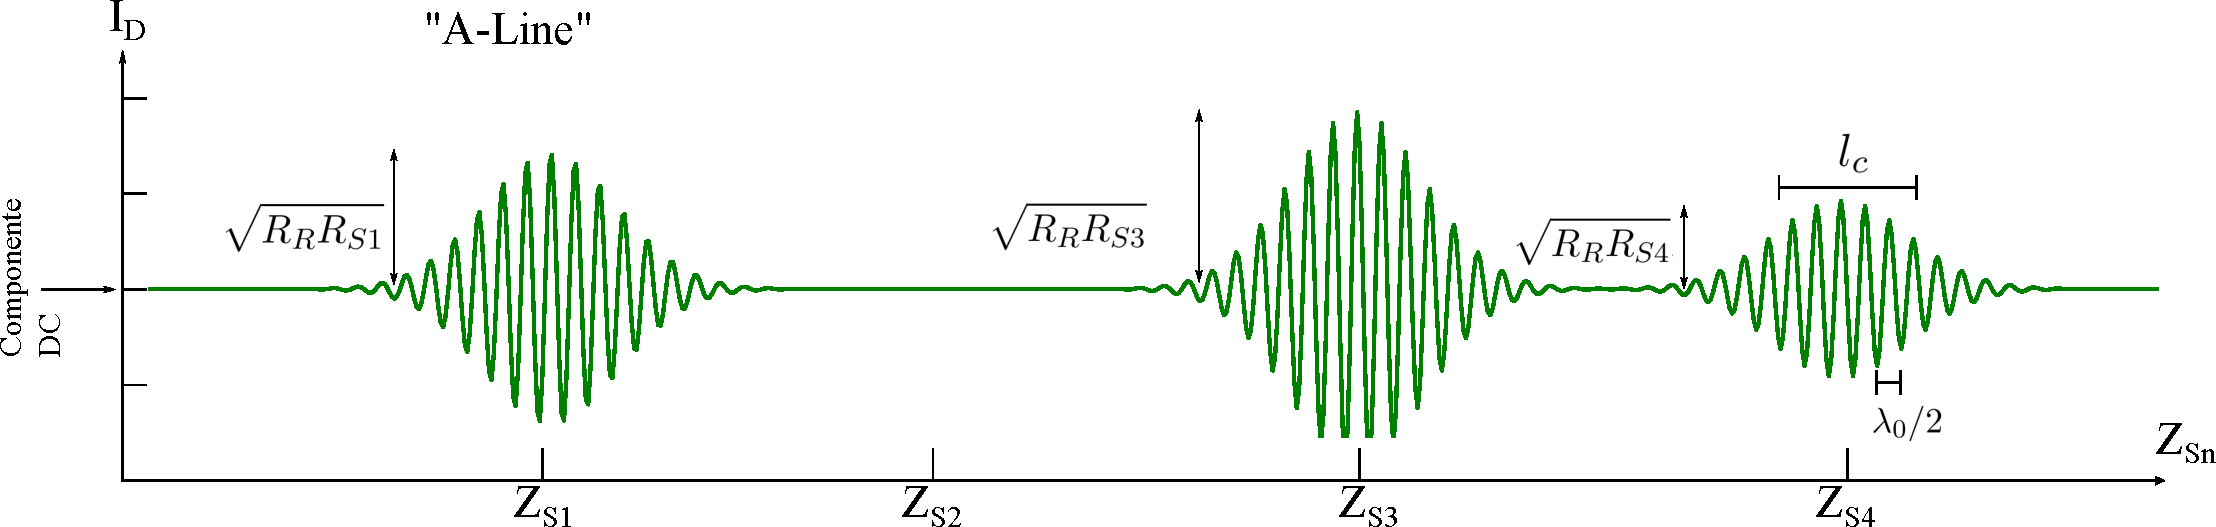
\includegraphics[width=\linewidth,keepaspectratio]{img/A_Line_1Gen}
	\caption{Línea A obtenida cuando se realiza el escaneo a una muestra con cuatro reflectores. La magnitud de la interferencia es lo que se busca medir mediante OCT.}
	\label{fig:tdoct}
\end{figure}


\subsection{Interferometría de baja coherencia en el dominio de Fourier}

En OCT del dominio de Fourier FDOCT (\textit{Fourier-domain optical coherence tomography}), la fotocorriente dependiente del número de onda $I_D(k)$ de la Eq.~\ref{eq:ID_fin} se captura y procesa mediante un análisis de Fourier que permite determinar el perfil de reflectividad $\sqrt{R_S(z_S)}$ de la muestra. En este proceso, el espejo de referencia se mantiene en una posición fija, mientras que las diferentes longitudes de onda son las encargadas de aportar la información de las diferentes profundidades en la muestra. En esta categoría hay dos divisiones para OCT, por un lado se encuentra  la tomografía óptica de coherencia en el dominio espectral SDOCT (\textit{spectral-domain optical coherence tomography}) o tomografía óptica de coherencia basada en espectrómetro. La OCT en el dominio espectral se basa en el empleo de una fuente de luz con banda ancha, con la diferencia de ubicar un espectrómetro en la salida del interferómetro, y todas las componentes frecuenciales de $I_D(k)$ se capturan de manera simultánea. Por otro lado, está la tomografía óptica de coherencia de fuente de barrido SSOCT (\textit{swept-source optical coherence tomography}), llamada también imagen óptica en el dominio frecuencial OFDI (\textit{optical frequency-domain imaging}). En este caso, las componentes espectrales de $I_D(k)$ se obtienen de forma secuencial, capturando la señal de una banda angosta, mientras que la fuente realiza un barrido por las diferentes longitudes de onda.

El perfil de reflectividad de la muestra $r_S(z_S)$ se calcula mediante la transformada inversa de Fourier de la corriente en el fotodetector, tomando en cuenta que la transformada de Fourier de un coseno es $\cos(kz_0) \rightleftarrows 1/2[\delta(z\pm z_0)]$ y la convolución entre funciones se define como el producto de sus transformadas de Fourier $x(z) \otimes y(z) \rightleftarrows X(k)Y(k)$; la transformada inversa de la Eq.~\ref{eq:ID_fin} corresponde a

\begin{align}
\label{eq:i_D_1}
i_D(z) &= \frac{\rho}{8}\left[\gamma (z) [R_R + R_{S1} + R_{S2} + ...] \right]\\ \notag
&+ \frac{\rho}{4} \left[\gamma (z) \otimes \sum_{n=1}^{N} \sqrt{R_R R_{S_n}}\{\delta[z\pm (2(z_R-z_{S_n}))]\}\right]\\
&+ \frac{\rho}{8} \left[\gamma (z) \otimes \sum_{m\neq n = 1}^{N} \sqrt{R_{s_n}R_{s_m}} \{\delta [z\pm 2(z_{S_n} - z_{S_m})]\} \right].\notag
\end{align}

\noindent La convolución de la función $\delta$ con la función coseno se puede calcular mediante sus propiedades, de manera que la Eq.~\ref{eq:i_D_1} corresponde a

\begin{align}
\label{eq:i_D_2}
i_D(z) &= \frac{\rho}{8}\left[\gamma (z) [R_R + R_{S1} + R_{S2} + ...] \right]\\ \notag
&+ \frac{\rho}{4} \left[\sum_{n=1}^{N} \sqrt{R_R R_{S_n}}\{\gamma [2(z_R - z_{S_n}) ] + \gamma[-2(z_R - z_{S_n}) ]\}  \right]\\
&+ \frac{\rho}{8} \left[ \sum_{m\neq n = 1}^{N} \sqrt{R_{S_n}R_{S_m}} \{\gamma [2(z_{S_n} - z_{S_m}) ] + \gamma[-2(z_{S_n} - z_{S_m}) ]\}  \right].\notag
\end{align}

\noindent La Eq.~\ref{eq:i_D_2} es una discretización de la función gaussiana correspondiente a las posiciones de los reflectores de la muestra, lo que se ha denominado línea A (Fig.~\ref{fig:fdoct}).
\begin{figure}[ht!]
	\centering
	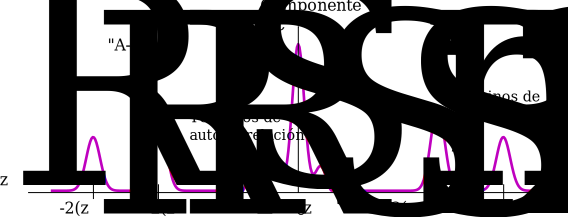
\includegraphics[width=\linewidth]{img/A_Line_FFT}
	\caption{Línea A obtenida en una medición de OCT en el dominio espectral.}
	\label{fig:fdoct}
\end{figure}

La función que se quiere recuperar $\sqrt{R_S(z_S)}$ en este caso se reproduce con las siguientes modificaciones, primero la distancia que se mide desde la posición de referencia está duplicada. El ancho de cada función $\delta$ está dado por la longitud de coherencia de la fuente. En la Eq.~\ref{eq:i_D_1} puede apreciarse claramente la convolución entre la muestra y la distribución de la fuente, esta definición corresponde a la función de dispersión de punto ($PSF$) en un sistema óptico convencional. Finalmente, la aparición de la segunda función $\delta$ se debe al complejo conjugado que resulta de la transformada de Fourier de la función coseno, en general, este término representa ruido en la información que se recupera, sin embargo, existe diferentes técnicas para solucionar este problema \cite{Ho2006,Vergnole2008}.


%\subsection{Interferometría de baja coherencia en el dominio del tiempo}
%
%En el caso de OCT en el dominio del tiempo TDOCT(\textit{time-domain optical coherence tomography}), el barrido no se realiza mediante el cambio del número de onda $k$, sino que a través de diferentes desplazamientos en el espejo de referencia $z_R$ se escanea la reflectividad de la muestra. En este proceso, a diferencia del caso anterior, hay una integración sobre todos los números de onda, de forma que la Eq.~\ref{eq:ID_fin} es convierte en
%
%\begin{align}
%%I_D(k) = &\frac{\rho}{4}S_0 [R_R+ R_{S1}+ R_{S2}+...]\\
%%&+\frac{\rho}{2}\left[ S_0 \sum_{n=1}^{N} \sqrt{R_R R_{S_n}} e^{[-z_R-z_{S_n}]^2 \Delta k^2}  \cos(2k_0 (z_R-Z_{S_n}))\right],
%\end{align}
%
%donde $S_0 = \int_{0}^{\infty} S(k) dk$, que es la energía emitida por la fuente. En este caso, nuevamente los términos que aparecen son una componente DC y una función gaussiana que en este caso se encuentra modulada por el coseno, cuya frecuencia depende de la longitud central de la fuente $k_0$ y la diferencia de camino entre los brazos, esto se ejemplifica en la Fig.~\ref{fig:tdoct}. La reflectividad de la muestra se puede encontrar entonces a través de la medida de la modulación que produce la señal portadora (la función coseno)  sobre la función gaussiana.
%
%\begin{figure}[h!]
%\centering
%-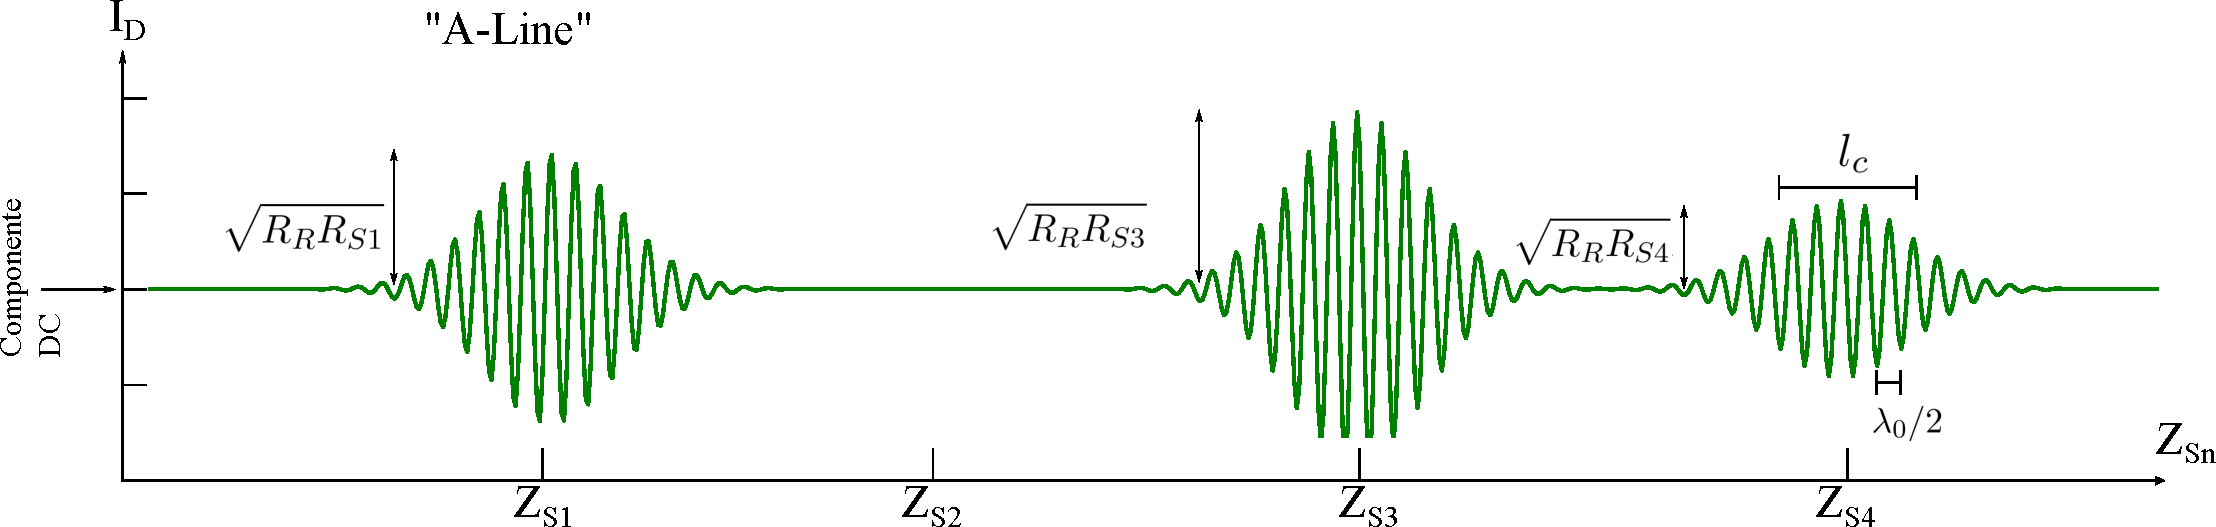
\includegraphics[width=\linewidth,keepaspectratio]{img/A_Line_1Gen}
%\caption{Línea A obtenida cuando se realiza el escaneo a una muestra con cuatro reflectores. La magnitud de la interferencia es lo que se busca medir mediante OCT.}
%\label{fig:tdoct}
%\end{figure}

%\subsection{La relevancia de la OCT en la investigación actual}

%En la actualidad, OCT se ha posicionado como una de las áreas de mayor interés, tanto científico, médico, como comercial. Para ejemplificar esto, en la Fig.~\ref{fig:oct_pub_by_year} se muestra la cantidad de publicaciones relacionadas a OCT desde su aparición hacia 1991. En la figura se aprecia como en los últimos años ha habido un crecimiento exponencial en la cantidad de artículos publicados en el tema, siendo la oftalmología y el estudio cardiovascular las principales áreas de publicación de OCT, datos tomados del US National Library of Medicine National Institutes of Health (http://www.ncbi.nlm.nih.gov/pubmed). Sin embargo, pese su gran expansión, desarrollo y estudio, en latinoamerica son pocos, los grupos de investigación acogen en sus líneas de investigación la OCT, para mostrar esto, en la Fig.~\ref{fig:oct_groups_map_png} se muestra la distribución global de los grupos que publican en OCT. En estos datos sobresalen grupos de universidades como Harvard, la Universidad de California y el MIT, datos tomados del US National Library of Medicine National Institutes of Health (http://www.ncbi.nlm.nih.gov/pubmed). Por último, el mercado de OCT se encuentra en crecimiento, como se indica en la Fig.~\ref{fig:oct_market}, en donde se aprecia que los ingresos de las compañías que producen equipos e indumentaria para OCT para el año 2015 cerró en alrededor de $800$ millones de dólares, lo que muestra un alto potencia para la comercialización e investigación en áreas relacionadas a la OCT, datos tomados del IOVS: Investigative Ophthalmology \& Visual Science.
%
%\begin{figure}[ht!]
%\centering
%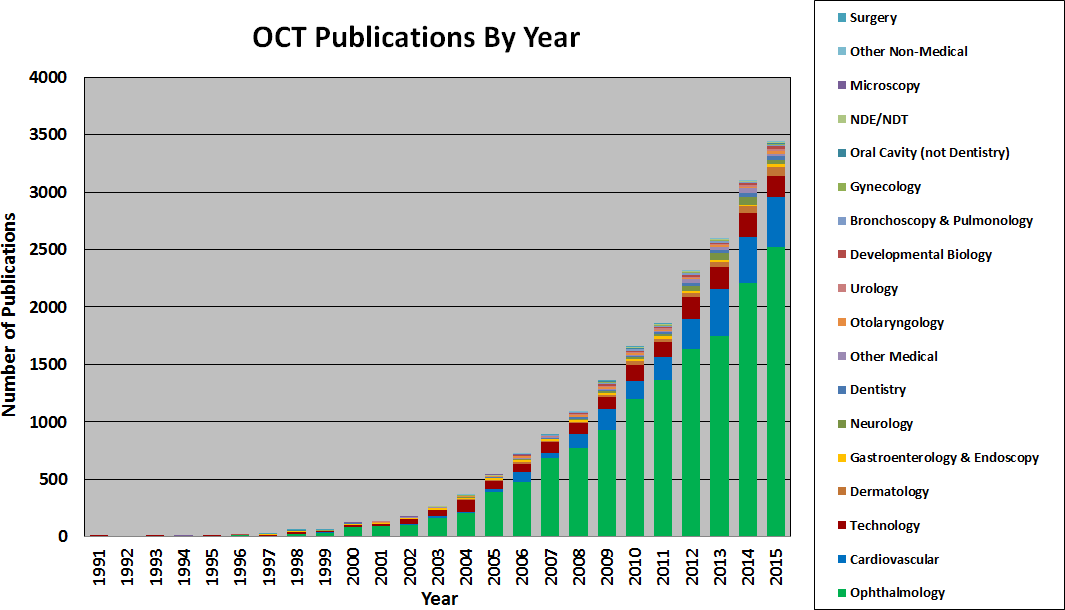
\includegraphics[width = \textwidth, keepaspectratio]{img/oct_pub_by_year.png}
%\caption[Citaciones sobre OCT en los últimos años.]{Citaciones sobre OCT en los últimos años. Tomado de http://www.ncbi.nlm.nih.gov/pubmed .}
%\label{fig:oct_pub_by_year}
%\end{figure}

%\begin{figure}[ht!]
%\centering
%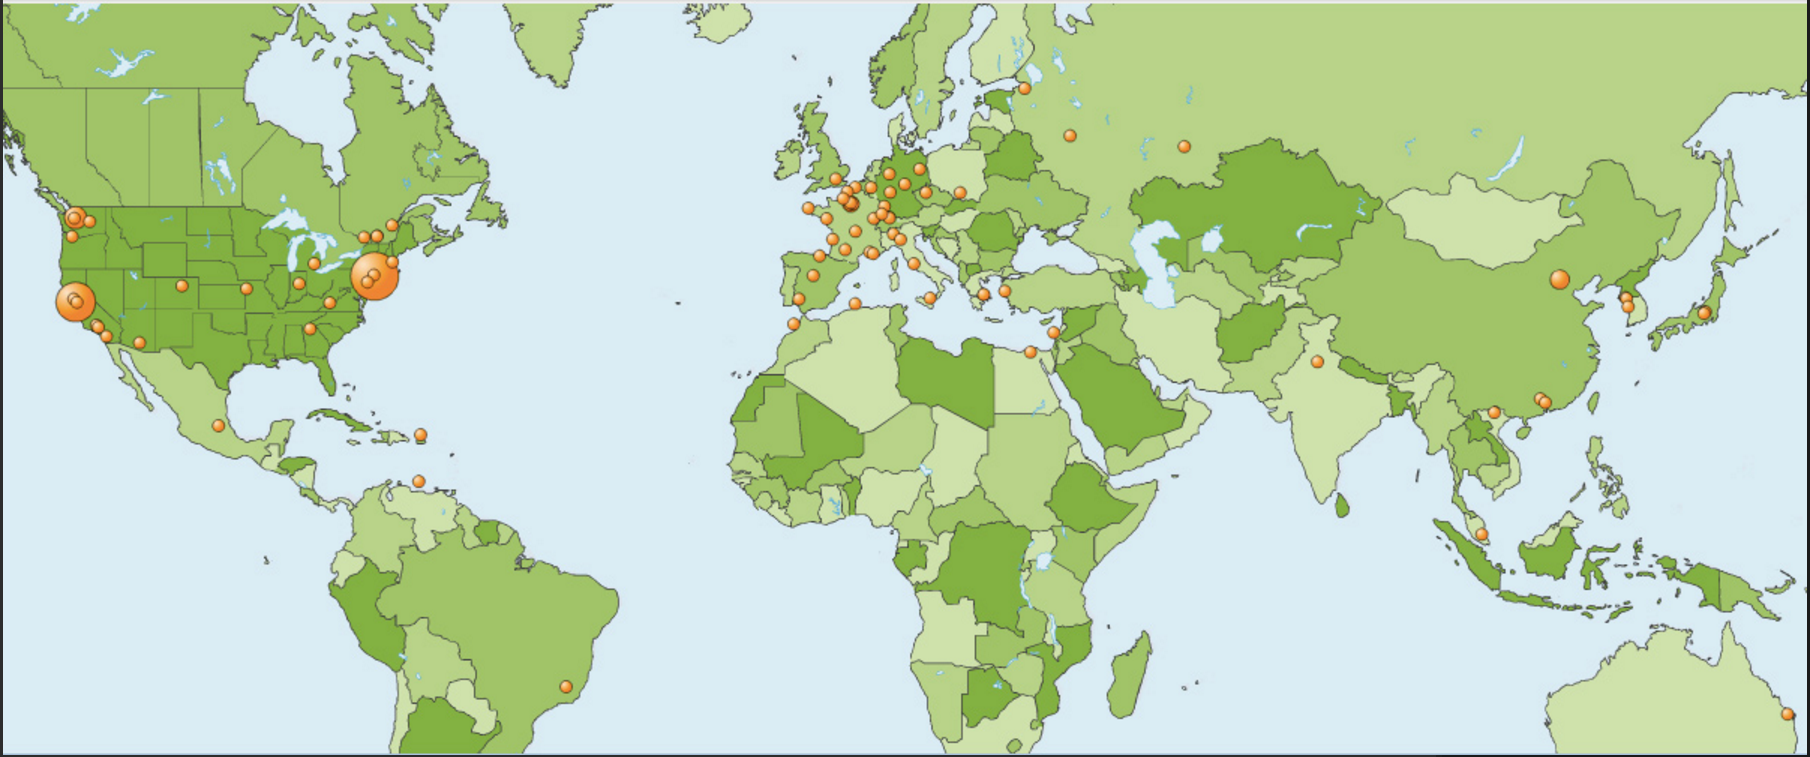
\includegraphics[width = \textwidth, keepaspectratio]{img/oct_groups_map_png.png}
%\caption[Mapa global de los grupos que investigan en OCT.]{Mapa global de los grupos que investigan en OCT. Tomada del Insihgt: OCT market http://www.sweptlaser.com/OCT-market .}
%\label{fig:oct_groups_map_png}
%\end{figure}

%\begin{figure}[ht!]
%\centering
%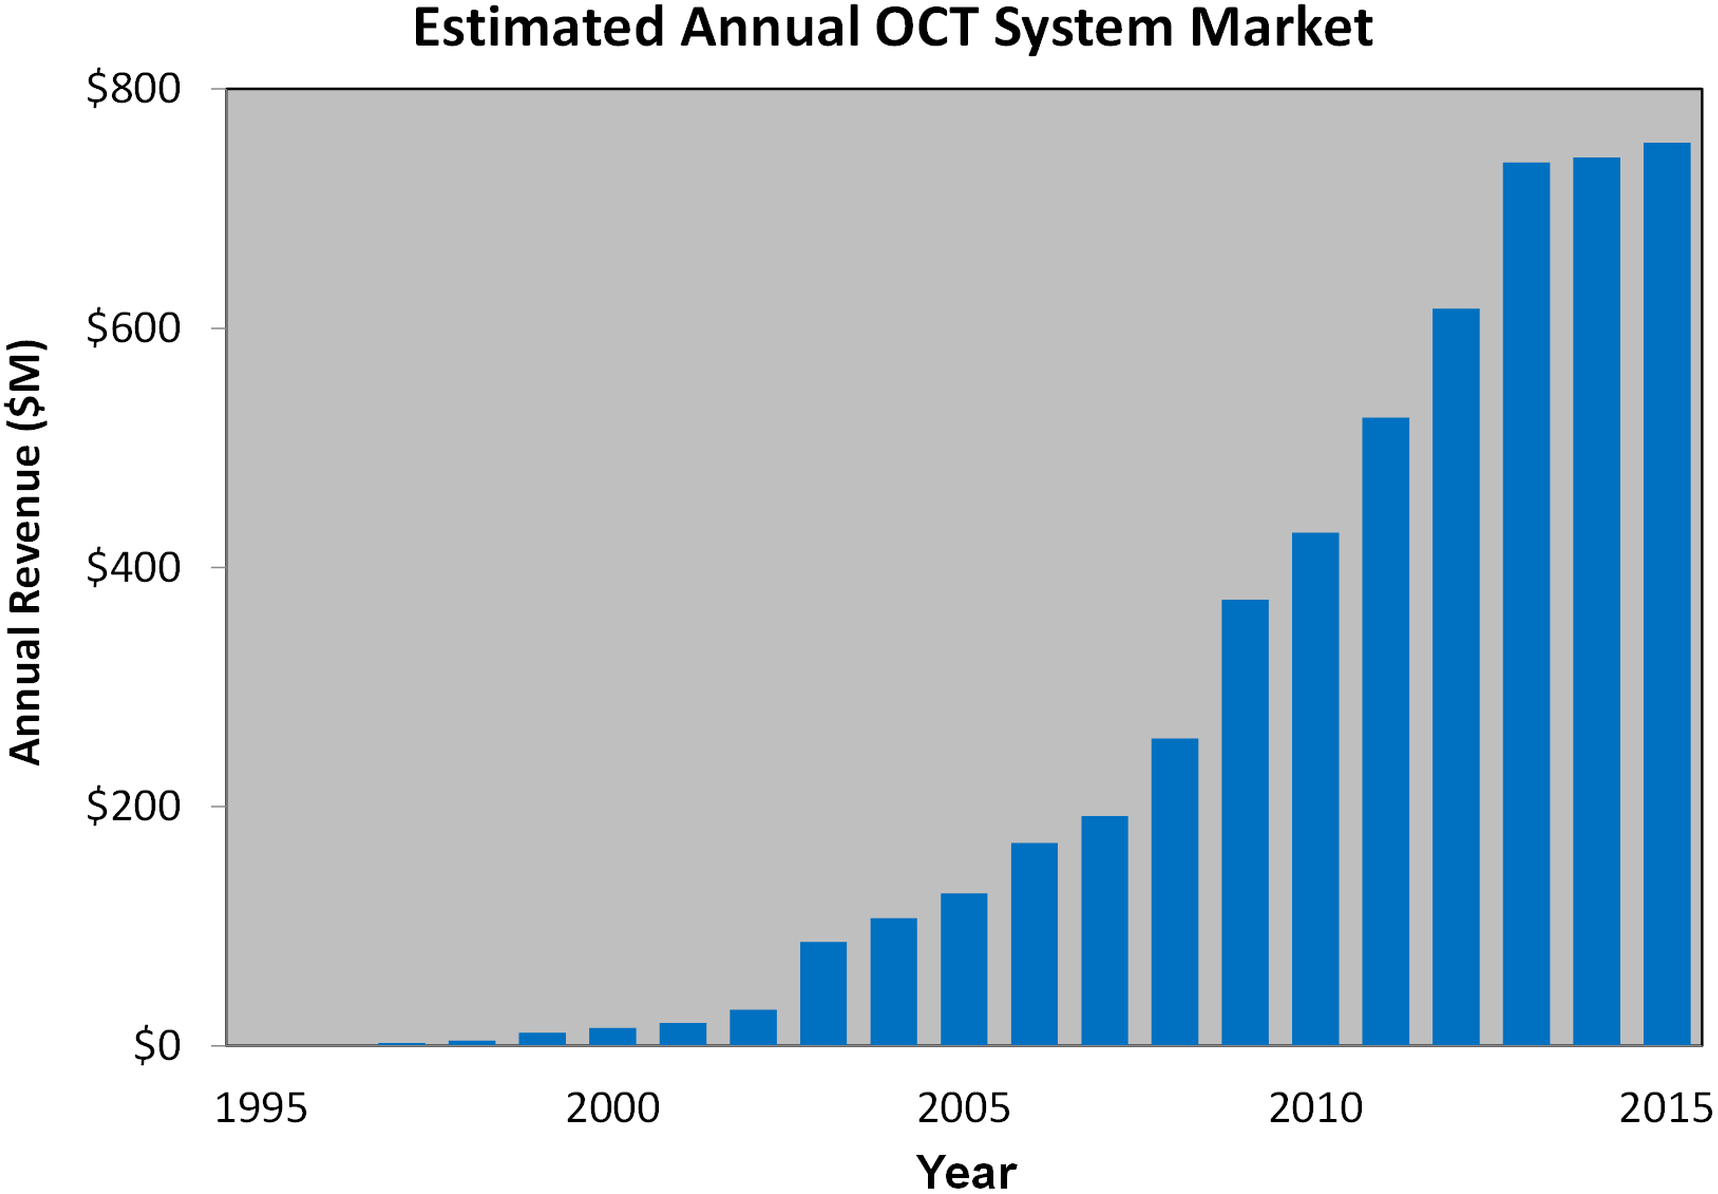
\includegraphics[width = \textwidth, keepaspectratio]{img/oct_market}
%\caption[Mercado de OCT.]{Mercado de la OCT en los últimos años, datos tomados de: http://iovs.arvojournals.org/.}
%\label{fig:oct_market}
%\end{figure}

%\subsection{Objetivos}
%\subsubsection{Objetivo general}
%
%%Desarrollar métodos de optimización en paralelo para la identificación de objetos de fase para la tomografía óptica coherente para diagnosis médico.
%%Mejorar la identificación de objetos de fase en tomografía óptica coherente mediante optimización en paralelo, que ayuden en el diagnosis médico.
%Estabilizar mediante posprocesamiento la fase en tomografía óptica de coherencia.
%
%\subsubsection{Objetivos específicos}
%
%\begin{itemize}
%	\item Identificar el estado de arte de la tomografía óptica coherente en aplicaciones biomédicas.
%%	\item Implementar un sistema óptico equivalente a los montajes utilizados durante la primera generación de la tomografía óptica coherente.
%	\item Implementar un sistema óptico de prueba de concepto de campo completo en la tomografía de coherencia óptica.
%%	\item Simular un volumen de datos que represente un objeto característico encontrados en la tomografía óptica coherente.
%%	\item Simular un volumen de datos que posea las características de los objetos que se pueden encontrar en la tomografía óptica coherente, incluyendo las corrupciones de fase provenientes del muestreo.
%	\item Realizar una simulación del muestreo y la formación de imagen en tomografía óptica de coherencia, incluyendo elementos de corrupción de fase.
%%	\item Desarrollar y aplicar un método de optimización de fase que permita encontrar las características del objeto simulado anteriormente.
%	\item Desarrollar un método de optimización de fase que permita recuperar el mapa de corrupción de la imagen simulada anteriormente.
%%	\item Definir una métrica del error para evaluar la convergencia del algoritmo de optimización propuesto.
%	\item Comprobar experimentalmente la funcionalidad del algoritmo propuesto con datos experimentales suministrados por el \emph{Wellman Center for Photomedicine, Harvard Medical School and Massachusetts General Hospital}.
%\end{itemize}


%\section{Conclusión}

